%%%%%%%%%%%%%%%%%%%%%%%%%%%%%%%%%%%%%%%%%%%%%%%%%%%%%%%%%%%%%%%%%%%%%%%%%%%%%
%	E-Yantra, IIT-Bombay

%	Document Author: Bhumika Varshney
%	Date: 1st July,2015

%%%%%%%%%%%%%%%%%%%%%%%%%%%%%%%%%%%%%%%%%%%%%%%%%%%%%%%%%%%%%%%%%%%%%%%%%%%%%

\documentclass[table,10pt,red]{beamer} 
% change the alerted colour to blue
\setbeamercolor{alerted text}{fg=blue}

\usetheme{Berlin}
% theme split

\usepackage{beamerthemesplit}
%\usepackage{xcolor}
\usepackage{booktabs,array}
\usepackage{listings}
\usepackage{hyperref}
\usepackage{verbatim,moreverb}
\usepackage{tikz}
\usepackage{colortbl}
\usepackage{multirow}
\usepackage{graphicx}
\usepackage{tikz}
\usetikzlibrary{arrows}



% theme shadow
\usepackage{beamerthemeshadow}

% For including figures
\usepackage{graphicx}

% logo
\logo{
\includegraphics[height=1cm]{iitblogo.pdf}}


% sf family, bold font
\sffamily \bfseries
% Beginning of title page
\title
% content inside [] appears at bottom of all page. content inside {} appears on first page as title. double backslash means line change 
[
	Firebird LPC2148 Robotics Research Platform	% bottom
	\hspace{0.5cm}
	\insertframenumber/\inserttotalframenumber
]
{
	Interrupts On Firebird-V Robot
}

\author
[
	www.e-yantra.org
]
{
	e-Yantra Team \\
  Embedded Real-Time Systems Lab\\
  Indian Institute of Technology-Bombay \\
}
\date
{
IIT Bombay \\ {\today}
}
 
 
\begin{document} 

% Slide-1: Title Page
\begin{frame}
	\titlepage
\end{frame} 

% Slide-2: Agenda for Discussion
\section*{Outline}
\begin{frame}[shrink=4]
	\frametitle{Agenda for Discussion}
	\tableofcontents
\end{frame} 


\section{Interrupts}
\subsection{What is an Interrupt}
	\begin{frame}
		\frametitle{What is an Interrupt} \pause
		\begin{enumerate}[$\checkmark$]
			\item<+-|alert@+> Any signal that causes break in continuity of some ongoing process \\[10pt]
			\item<+-|alert@+> In microcontrollers interrupt signal halts the execution of main program and dedicates processor to another task \\[10pt]
			\item<+-|alert@+> While main program is running, if an interrupt occurs, execution of main program is stopped, and program counter goes to address of ISR \\[10pt]  
			\item<+-|alert@+> Interrupt Service Routine: Program that needs to be executed when interrupt occurs \\[10pt]
			\item<+-|alert@+> After program inside ISR is executed completely, program counter returns back to point where main program was interrupted \\[10pt]
		\end{enumerate}  
	\end{frame}
	
%\subsection{Interrupt Program Execution}
%\begin{frame}
%	\frametitle{Normal program execution}
%	\centering
%	\begin{tabular}{|c|c||c|c|c|}
%	\multicolumn{2}{|c||}{\textbf{SP}} & \textbf{PC} & & \textbf{Main Program} \pause \\[10pt]
%	
%	0x80 & 0x*** \pause & 0x0101 & \begin{tikzpicture} \draw[->][thick,red,line width = 0.1cm] (0,0.2)--(0.5,0.2); \end{tikzpicture} \pause& {Reqd=Distance/5.44;} \pause \\[10pt]
%	
%	0x80 & 0x*** \pause & 0x0102 & \begin{tikzpicture} \draw[->][thick,red,line width = 0.1cm] (0,0.2)--(0.5,0.2); \end{tikzpicture}\pause & int1setup(); \pause \\[10pt]
%	
%	0x80 & 0x*** \pause&  0x0103 & \begin{tikzpicture} \draw[->][thick,red,line width = 0.1cm] (0,0.2)--(0.5,0.2); \end{tikzpicture}\pause & while(reqd<count); \pause \\[10pt]
%
%	0x80 & 0x*** & \pause 0x0104 & \begin{tikzpicture} \draw[->][thick,red,line width = 0.1cm] (0,0.2)--(0.5,0.2); \end{tikzpicture}\pause & stop(); \pause \\[10pt]
%	
%	\end{tabular}
%\end{frame}

%\begin{frame}[shrink = 5]
%	\frametitle{ISR program execution}
%	\scriptsize{
%	\centering
%	\begin{tabular}{|c|c||c|c|c|c}
%		\multicolumn{2}{|c||}{\textbf{SP}} & \textbf{PC} & & \textbf{Main Program} \pause \\[10pt]
%	
%	0x80 & 0x*** \pause & 0x0101 & \begin{tikzpicture} \draw[->][thick,red,line width = 0.1cm] (0,0.2)--(0.5,0.2); \end{tikzpicture} \pause& {Reqd=Distance/5.44;} \pause \\[10pt]
%	
%	0x80 & 0x*** \pause & 0x0102 & \begin{tikzpicture} \draw[->][thick,red,line width = 0.1cm] (0,0.2)--(0.5,0.2); \end{tikzpicture}\pause & int1setup(); \pause \\[10pt]
%	
%	0x80 & 0x*** \pause&  0x0103 & \begin{tikzpicture} \draw[->][thick,red,line width = 0.1cm] (0,0.2)--(0.5,0.2); \end{tikzpicture}\pause & while(reqd<count); \pause & \begin{tikzpicture} %\draw[<-][thick,red,line width = 0.1cm] (0,0.2)--(0.5,0.2); \end{tikzpicture} INT1 (0x0013) \pause \\[10pt]

%	\onslide<16-> 0x81 & \onslide<15->0x0104 &  \onslide<14> \begin{tikzpicture} \draw[<-][thick,red,line width = 0.1cm] (0,0.2)--(0.5,0.2); \end{tikzpicture}  \onslide<13-14> 0x0104  & \pause &  \pause %\\[10pt] \pause \pause
%	
%	0x81 & 0x0104 & 0x0013 & \begin{tikzpicture} \draw[->][thick,red,line width = 0.1cm] (0,0.2)--(1,0.2); \end{tikzpicture}& \onslide<18> & Left Shaft Count++ \pause \\[10pt]
	
	
	
%	\end{tabular}
%	}
%\end{frame}


\subsection{Closed Loop Programming}
\begin{frame}[shrink=2]
	\frametitle{Closed Loop Programming} \pause
	\begin{itemize}
		\item<+-|alert@+> Systems that utilize feedback are called closed-loop control systems  \pause \\[10pt] 
		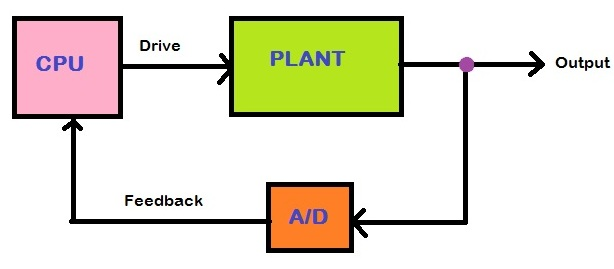
\includegraphics[width =\linewidth]{closed_loop_feedback} \pause \\[10pt]
		\item<+-|alert@+> The feedback is used to make decisions about changes to the control signal that drives the plant \\[10pt]
		\item<+-|alert@+> An open-loop control system doesn't have or doesn't use feedback \\[10pt]
	\end{itemize}
\end{frame}

\section{Interrupt-Handling on Firebird}
\subsection{Sources of Interrupt}
\begin{frame}
		\frametitle{Sources of Interrupt on LC2148}\pause
			LPC2148 has \textbf{Twenty-One} Different sources for Interrupt generation \pause \\[8pt]
			\begin{itemize}
				\item <3-> Timer Overflow Interrupt \\[8pt]
				\item <4-> Timer Compare \\[8pt]
				\item <5-> Serial interrupt \\[8pt]
				\item <6-> Wired \& Wireless Interrupt \\[8pt]
				\item <7-> External hardware Interrupt  \\[8pt]	
				\item <8-> RTC Interrupt  \\[8pt]
				\item <9-> I2C Interrupt  \\[8pt]
				\item <10-> WDT Interrupt  \\[8pt]
			\end{itemize}\pause
\end{frame}
\begin{frame}
	\frametitle{Sources of Interrupt on LPC2148}\pause
	Interrupts in LPC2148 are handled by \textbf{Vectored Interrupt Controller(VIC)} and are classified into 3 types based on the priority levels.(Though Interrupts can classified in many different ways as well) \\[12pt] \pause
	\begin{enumerate}
		\item \textbf{Fast Interrupt Request i.e FIQ:} which has highest priority \\[5pt] \pause
		\item \textbf{Vectored Interrupt Request i.e Vectored IRQ :} which has 'middle' or priority between FIQ and Non-Vectored IRQ. \\[5pt] \pause
		\item \textbf{Non-Vectored IRQ :} which has the lowest priority. \\[5pt] \pause
	\end{enumerate} 
	 The Vectored Interrupt Controller (VIC) takes 32 interrupt request inputs. \pause
\end{frame}
\subsection{Position Encoder}
	\begin{frame}[shrink = 8.9] 
		\frametitle{Position encoder} \pause
			\begin{minipage}[c]{0.4\textwidth}
				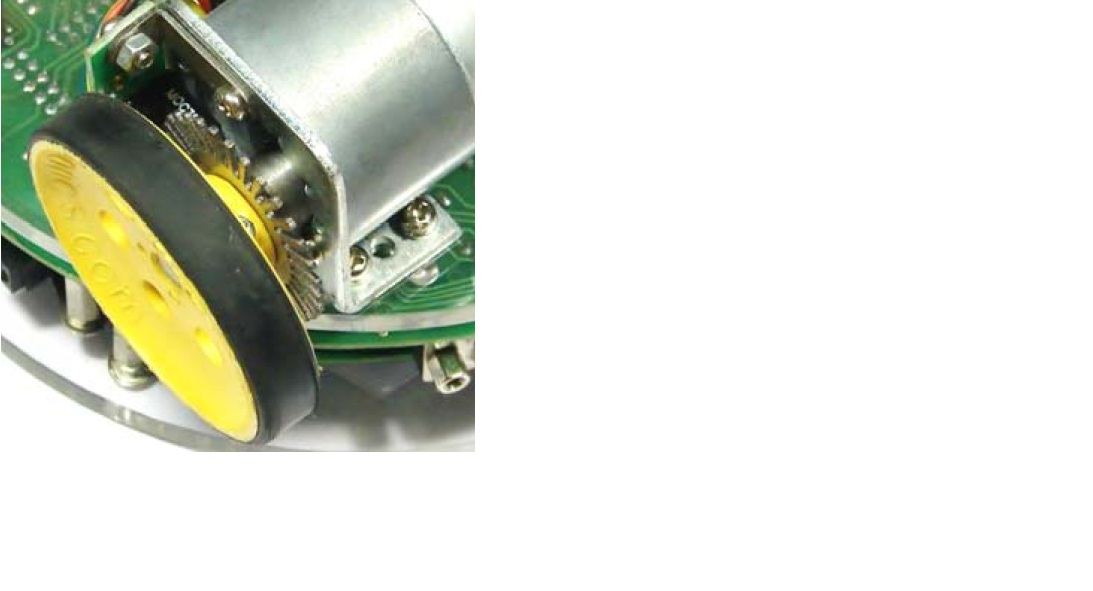
\includegraphics[width = 1.5\linewidth]{encoder_on_fb}\pause\\[10pt]
				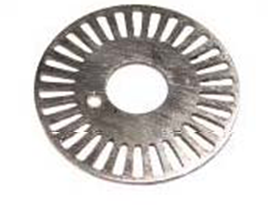
\includegraphics[width = 0.8\linewidth]{slotted_disk}\\%[10pt]
			\end{minipage}
			\pause
			\hfill
			\begin{minipage}[c]{0.5\textwidth}
				\begin{enumerate}
					\item <+-|alert@+> Optical position encoders are used for position feedback \\[5pt]
					\item <+-|alert@+> It consists of IR LED and photo diode placed opposite of each other \\[5pt]
					\item <+-|alert@+> When IR light is interrupted by encoder disc,its output state changes (high to low or low to high)\\[5pt]
					\item <+-|alert@+> Output of the encoder is connected to the interrupt pin of the microcontroller\\[5pt]
					\item <+-|alert@+> Left encoder is connected to EINT3 and  Right encoder is connected to EINT0 \\[5pt]
				%	\item <+-|alert@+> Right encoder is connected to INT5\\[6pt]
				\end{enumerate}
			\end{minipage}
	\end{frame}
	
\subsection{Interrupt Calculation}
	\begin{frame}
		\frametitle{Some Mathematics...}\pause
			\begin{enumerate}
				\item <+-|alert@+> Number of slots in disc \color{red}= 30 \color{black}\\[10pt]
				\item <+-|alert@+> Number of Pulse/rotation \color{red} = 30 \color{black}\\[10pt]
				\item <+-|alert@+> Diameter of wheel \color{red} = 52mm \color{black} \\[10pt]
				\item <+-|alert@+> Resolution of position encoder \\[5pt] \pause 
					\hspace{50pt}	\color{red} = ($\pi*$d)/30 = 5.44 \color{black}	\pause		
				\item <+-|alert@+> Pulse count \\[10pt]\
					\hspace{50pt}	\color{red} = distance/5.44 \color{black}
			\end{enumerate}
	\end{frame}
	

\subsection{External Interrupt Initialization}
	\begin{frame}
		\frametitle{Initialization} 
		To setup Interrupts for right and left position encoders, few registers are required to initialize:  \pause
		\begin{itemize}
			\item EXTMODE - External Interrupt Mode Register\pause
			\item EXTPOLAR - External Interrupt Polarity Register\pause
			\item VICIntSelect - Interrupt Select Register\pause
			\item VICVectCntl - Vector Control Register \pause
			\item VICVectAddr - Vector Address Register \pause
			\item EXTINT - External Interrupt flag Register\pause
			\item VICIntEnable - Interrupt Enable Register\pause
			
		\end{itemize} 
	\end{frame}
	
\begin{frame}
		\frametitle{EXTMODE- External Interrupt Mode Register}
		\begin{itemize}
			\item This register is Used to control whether external interrupt is edge or level sensitive \pause 
		\end{itemize} 
		\centering
		\begin{tabular}{!{\vrule width 0.8pt}>{\columncolor[gray]{0.9}[0.8\tabcolsep]}c|>{\columncolor[gray]{0.9}[0.8\tabcolsep]}c|>{\columncolor[gray]{0.9}[0.8\tabcolsep]}l|>{\columncolor[gray]{0.9}[0.8\tabcolsep]}c!{\vrule width 0.8pt}}
			\noalign{\hrule height 0.5pt}
			Bit & Symbol & Description & Bit Value  \\  
			\noalign{\hrule height 1pt} 
			\vspace{2pt} 
			7 & - & Reserved &  0  \\
			\vspace{2pt}
			6 & - & Reserved &  0  \\
			\vspace{2pt}
			5 & - & Reserved &  0  \\
			\vspace{2pt}
			4 & - & Reserved &  0 \\
			\vspace{2pt}
			3 & EXTMODE3 & To select EINT3 as edge or level sensitive & \color{red}1\color{black} \\
			\vspace{2pt}
			2 & EXTMODE2 & To select EINT2 as edge or level sensitive & 0 \\
			\vspace{2pt}
			1 & EXTMODE1 & To select EINT1 as edge or level sensitive & 0 \\
			\vspace{2pt}
			0 & EXTMODE0 & To select EINT0 as edge or level sensitive & \color{red}1\color{black} \\
			\noalign{\hrule height 0.5pt}			
		\end{tabular}	\pause \\[10pt]
		\hspace{8cm}EICRA\hspace{1pt}=\hspace{1pt}\color{red}0x00 \color{black}
	\end{frame}
	
	\begin{frame}
		\frametitle{EXTPOLAR- External Interrupt Polarity Register}
		\begin{itemize}
			\item This register is Used to control which level(high or low) or edge(rising or falling) on each pin will cause an interrupt \\[5pt] \pause 
		\end{itemize} 
		\centering
		\begin{tabular}{!{\vrule width 0.8pt}>{\columncolor[gray]{0.9}[0.8\tabcolsep]}c|>{\columncolor[gray]{0.9}[0.8\tabcolsep]}c|>{\columncolor[gray]{0.9}[0.8\tabcolsep]}l|>{\columncolor[gray]{0.9}[0.8\tabcolsep]}c!{\vrule width 0.8pt}}
			\noalign{\hrule height 0.5pt}
			Bit & Symbol & Description & Bit Value  \\  
			\noalign{\hrule height 1pt} 
			\vspace{2pt} 
			7 & - & Reserved &  0  \\
			\vspace{2pt}
			6 & - & Reserved &  0  \\
			\vspace{2pt}
			5 & - & Reserved &  0  \\
			\vspace{2pt}
			4 & - & Reserved &  0 \\
			\vspace{2pt}
			3 & EXTPOLAR3 & EINT3 as falling edge sensitive & 0 \\
			\vspace{2pt}
			2 & EXTPOLAR2 & EINT2 as falling edge sensitive & 0 \\
			\vspace{2pt}
			1 & EXTPOLAR1 & EINT1 as falling edge sensitive & 0 \\
			\vspace{2pt}
			0 & EXTPOLAR0 & EINT0 as falling edge sensitive & 0 \\
			\noalign{\hrule height 0.5pt}			
		\end{tabular}	\pause \\[6pt]
		EXTPOLAR\hspace{1pt}=\hspace{1pt}\color{red}0x00 \color{black};
	\end{frame}
	
	\begin{frame}
		\frametitle{EXTINT- External Interrupt Flag Register}
		\begin{itemize}
			\item When Interrupt occurs, corresponding bit of this register becomes high. To clear it, write 1 to that bit. \pause 
		\end{itemize} 
		\centering
		\begin{tabular}{!{\vrule width 0.8pt}>{\columncolor[gray]{0.9}[0.8\tabcolsep]}c|>{\columncolor[gray]{0.9}[0.8\tabcolsep]}c|>{\columncolor[gray]{0.9}[0.8\tabcolsep]}l|>{\columncolor[gray]{0.9}[0.8\tabcolsep]}c!{\vrule width 0.8pt}}
			\noalign{\hrule height 0.5pt}
			Bit & Symbol & Description & Bit Value  \\  
			\noalign{\hrule height 1pt} 
			\vspace{2pt} 
			7 & - & Reserved &  0  \\
			\vspace{2pt}
			6 & - & Reserved &  0  \\
			\vspace{2pt}
			5 & - & Reserved &  0  \\
			\vspace{2pt}
			4 & - & Reserved &  0 \\
			\vspace{2pt}
			3 & EINT3 & indicate EINT3 interrupt occurence  & \color{red}1\color{black} \\
			\vspace{2pt}
			2 & EINT2 & indicate EINT2 interrupt occurence & 0 \\
			\vspace{2pt}
			1 & EINT1 & indicate EINT1 interrupt occurence & 0 \\
			\vspace{2pt}
			0 & EINT0 & indicate EINT0 interrupt occurence & \color{red}1\color{black} \\
			\noalign{\hrule height 0.5pt}			
		\end{tabular}	\pause \\[6pt]
		EXTINT\hspace{1pt}=\hspace{1pt}\color{red}0x09 \color{black};
	\end{frame}
	
\begin{frame}
		\frametitle{VICIntSelect- Interrupt Select Register}
		\begin{itemize}
			\item[$\bullet$] This register classifies each of the 32 interrupt requests as contributing to FIQ or IRQ.Writing 1 to any bit contributes to FIQ and writing 0 contributes to IRQ. 
		\end{itemize}  \pause 
			\footnotesize
			\begin{tabular}{|c|c|c|c|c|c|c|c|c|c|}
				\hline Bit & 31-23 & 22 & 21 & 20 & 19 & 18 & 17 & 16 & 15 \\ 
				\hline Symbol & - & USB & AD1 & BOD & I2C1 & ED0 & EINT3 & EINT2 & EINT1 \\ 
				\hline 
			\end{tabular}
			\\[10pt]
			\begin{tabular}{|c|c|c|c|c|c|c|c|c|}
				\hline Bit & 14 & 13 & 12 & 11 & 10 & 9 & 8 & 7\\ 
				\hline Symbol & EINT0 & RTC & PLL & SPI1/SSP & SPI0 & I2C0 & PWM0 & UART1 \\ 
				\hline 
				\end{tabular}
				\\[10pt]
				\begin{tabular}{|c|c|c|c|c|c|c|c|}
					\hline Bit & 6 & 5 & 4 & 3 & 2 & 1 & 0 \\ 
					\hline Symbol & UART0 & TIMER1 & TIMER0 & ARMCore1 & ARMCore0 & - & WDT \\ 
					\hline 
					\end{tabular} 
					\\[10pt]
					\small
		VICIntSelect\hspace{1pt}=\hspace{1pt}\color{red}0x00000000 \color{black};
	\end{frame}

\begin{frame}
	\frametitle{VICIntEnable- Interrupt Enable Register}
	\begin{itemize}
		\item[$\bullet$] This register classifies each of the 32 interrupt requests as contributing to FIQ or IRQ. Writing 1 to any bit enables the corresponding interrupt. 
	\end{itemize}  \pause 
	\footnotesize
	\begin{tabular}{|c|c|c|c|c|c|c|c|c|c|}
		\hline Bit & 31-23 & 22 & 21 & 20 & 19 & 18 & 17 & 16 & 15 \\ 
		\hline Symbol & - & USB & AD1 & BOD & I2C1 & ED0 & EINT3 & EINT2 & EINT1 \\ 
		\hline 
	\end{tabular}
	\\[10pt]
	\begin{tabular}{|c|c|c|c|c|c|c|c|c|}
		\hline Bit & 14 & 13 & 12 & 11 & 10 & 9 & 8 & 7\\ 
		\hline Symbol & EINT0 & RTC & PLL & SPI1/SSP & SPI0 & I2C0 & PWM0 & UART1 \\ 
		\hline 
	\end{tabular}
	\\[10pt]
	\begin{tabular}{|c|c|c|c|c|c|c|c|}
		\hline Bit & 6 & 5 & 4 & 3 & 2 & 1 & 0 \\ 
		\hline Symbol & UART0 & TIMER1 & TIMER0 & ARMCore1 & ARMCore0 & - & WDT \\ 
		\hline 
	\end{tabular} 
	\\[10pt]
	\small
	VICIntEnable\hspace{1pt}=\hspace{1pt}\color{red}0x00024000 \color{black};
\end{frame}

\begin{frame}
	\frametitle{VICVectCntl- Vector Control Registers0-15}
	\begin{itemize}
		\item There are total 16 vector control registers. Each of these registers controls one of the 16 vectored IRQ slots. VICVectCntl0 has the highest priority and VICVectCntl15 the lowest. \pause \\[8pt] 
	\end{itemize} 
	\centering
	\small
	\begin{tabular}{|c|c|l|c|}
		\hline
		Bit & Symbol & Description & Bit Value  \\
		\hline  
		31-6 & - & Reserved &  0  \\
		\hline
		\multirow{2}{*}{5} & \multirow{2}{*}{IRQslot\_en}  & When 1, this vectored IRQ & \multirow{2}{*}{\color{red}1\color{black}} \\
		                   &                               & slot is enabled &    \\
		\hline
		\multirow{2}{*}{4-0} & int\_request/ & The number of the interrupt &  \multirow{2}{*}{Interrupt number}  \\
		                     & sw\_int\_assig & request assigned to this slot & \\
		\hline
	\end{tabular}	\pause \\[8pt]
	VICVectCntlx\hspace{1pt}=\hspace{1pt}\color{red}0x20$|$Interrupt number \color{black}
\end{frame}		

\begin{frame}
	\frametitle{VICVectAddr- Vector Address Registers0-15}
	\begin{itemize}
		\item These registers hold the addresses of the	Interrupt Service routines (ISRs) for the 16 vectored IRQ slots. \pause \\[5pt] 
	\end{itemize} 
	\hspace{1cm}VICVectCntlx\hspace{1pt}=\hspace{1pt}\color{red}0x20$|$Interrupt number \color{black}\\[5pt]
	\begin{block}<2->{\textbf{For Example:}}\pause
		\begin{semiverbatim}
			\small
			 To set EINT3(left encoder) at highest priority and EINT0(right encoder) at lower priority, combination of both VICVectCntl and VICVectAddr registers are used as follows - \newline 
			\color{red} VICVectCntl0 = 0x20$|$17; \newline
			            VICVectAddr0 = (int)IRQ\_Eint3; \newline
			            VICVectCntl1 = 0x20$|$14; \newline
			            VICVectAddr1 = (int)IRQ\_Eint0; \newline
		\end{semiverbatim} 
	\end{block}
	
\end{frame}

\subsection{ISR}
\begin{frame}[fragile]
		\frametitle{ISR-Interrupt Service Routine} \pause
			\textbf{The format of ISR for external interrupt is} \pause \\[20pt]
			
			\begin{block}<2->{ISR Format}\pause
				\begin{semiverbatim}
				\ \ __irq IRQ_Eint\color{red}n\color{black}
				\ \ \{
 			 \ \		code 		
 				\}
 				\end{semiverbatim} 
 			\pause Where n = External Interrupt Number (For LPC2148: n=0-4)
 			\end{block}			
\end{frame}

\subsection{C-Code}

\begin{frame}[shrink = 2,fragile]
	\frametitle{Syntax for C-Program} \pause
	\begin{itemize}
		\item Port Initialization
	\end{itemize}
		\begin{block}<1->{Left and Right Encoder Port Initialization}	\pause
		\begin{semiverbatim}
				\scriptsize{
							PINSEL1 = 0x20000001; \color{red}//Enabling P0.16 as EINT0  and P0.30 as EINT3\color{black}
						   }
			\end{semiverbatim}
		\end{block} \pause 
	\begin{itemize}
		\item Interrupt Initialization
	\end{itemize}
		\begin{block}<2->{Left and right Encoder Interrupt Initialization}	\pause
			\begin{semiverbatim}
					\scriptsize{
							EXTMODE = 0x09;	               \color{red}// EINT3 and EINT0 is edge sensitive\color{black}
							EXTPOLAR = 0x00;                \color{red}// EINT3 and EINT0 in triggered on falling edge\color{black}					
							VICIntSelect = 0x00000000;	     \color{red}// Setting EINT2 and EINt0 as IRQ(Vectored)\color{black}
							EXTINT = 0x09;                   \color{red}//Setting EINT2 \& EINT0 interrupt flag\color{black}
							VICIntEnable = (1<<17) | (1<<14); \color{red}// Enable EINT3 \& EINT0 flags\color{black}
						 }
			\end{semiverbatim}
		\end{block} \pause
\end{frame}

\begin{frame}
\hskip4cm
\textbf{\LARGE Thank You!} \\[20pt]
\hskip3cm
\scriptsize Post your queries on: 
\hyperref[www.e-yantra.org]{\color{blue} http://qa.e-yantra.org/ \color{black}} 
\end{frame}


\end{document} 